\section{Profiling and Testing}
\label{sec:profiling-and-testing}



\subsection{Testing Framework}

Testing a library like Grackle, with its mix of \texttt{Fortran}, and
\texttt{C++} code, can be difficult. In the interest of ultimately improving
test coverage and make it easier to prototype tests, Grackle employs a
python-based testing framework that makes heavy use of the \texttt{pygrackle}
python wrapper for the Grackle. The tests are orchestrated using the
\texttt{py.test}\footnote{http://pytest.org/} package.

Currently there are two different types of tests in the Grackle test suite: unit
tests and answer tests. A unit test in Grackle compares the results of a
calculation using Grackle to some set of ``correct'' answers that are known
\textit{a priori}. The unit tests currently implemented in grackle test that the
unit system is behaving correctly (see Section~\ref{sec:unit-test}) and that the
ionization equilibrium for a primordial gas agrees with the analytic prediction
using the rates implemented in Grackle (see Section~\ref{sec:primordial-test}).

The answer tests consist of a set of example calculations where each calculation
writes out a summary plot as well as an \texttt{hdf5} dataset that is loadable
by the \texttt{yt} package. Known ``correct'' answers for the summary plot and
\texttt{yt}-loadable dataset are saved in the repository so that code changes in
Grackle can be tested to ensure that andwers produced by the library do not
change. This process does not prevent \textit{incorrect} answers from being
generated initially, but it does prevent the answers from changing as the code
is developed. Incorrect answers are prevented by manually inspecting test
answers when the test is first added to the codebase. If subsequently a bug is
discovered and the test output changes, then the test answer must also be
manually updated. Currently Grackle contains answer tests calculations for the
cooling rate (see Section~\ref{sec:cooling-rate-test}) in a uniform density
cloud at a fixed time, a calculation of the density and temperature of a gas
cloud undergoing free-fall collapse (see Section~\ref{sec:free-fall-test}), and
a calculation for the temperature evolution of a uniform-density cloud (see
Section~\ref{sec:uniform-cooling-test}).  The answers test are run several times
using different input physics to ensure Grackle's solvers are well-exercised by
the tests.

\subsubsection{Unit Test: Unit Systems}
\label{sec:unit-test}

For a given set of physical conditions, (i.e., densities and internal
energies), the results of Grackle-related calculations should be
independent of the choice of reference frame (comoving or proper) and
internal unit system.  However, because chemistry and cooling
calculations involve numeric values that span many orders of
magnitude, round-off error will eventually lead to significant
differences when the internal unit systems are varied beyond a certain
degree.  The unit systems unit tests set up two fluid container
objects with the same physical conditions but different internal unit
systems.  In each instance, the chemical species fractions are evolved
until ionization equilibrium has been reached (see \S
\ref{sec:pyfluid}), after which time the cooling time is calculated.
The tests assert that the cooling time values agree to within 4
decimal places between the two unit systems.

Three variants of this unit test exist.  In the first two, a
comoving-frame unit system appropriate for a cosmological simulations
is compared with a proper-frame unit system drawn from a random number
generator that allows the density, time, and length units to vary by 4
orders of magnitude.  A cosmologically appropriate unit system is
roughly defined as one with density units equal to the average
comoving matter density of the Universe, $\bar{\rho}_{m}$; time units
proportional to 1/$\sqrt{G\ \bar{\rho}_{m}}$; and length units on the
scale of Mpc.  One of the two of these type is performed with the
non-equilibrium chemistry solver and the other with the fully
tabulated solver.  In both cases, we compare a randomly generated
proper-frame unit system with a comoving-frame unit system at z = 0
and z $>$ 0, where the proper and comoving frames differ.  In these
tests, a UV background model is also used as the radiative heating
rate is proportional to $\rho$, whereas collisional heating/cooling
rates are proportional to $\rho^{2}$ (or $\rho^{3}$ for three-body
reactions).  Including heating/cooling terms with different density
scaling is useful for exposing errors in adjusting between comoving
and proper reference frames.

The final variant of the unit system test compares two randomly
generated proper-frame unit systems whose density units differ by as
much as possible while maintaining equivalency to 4 decimal places.
In practice, we find that the density units can differ by roughly 31
orders of magnitude before the threshold level of accuracy is lost.
With this in mind, we allow the two randomly generated unit systems to
span 2 orders of magnitude with the center of each random distribution
chosen such that the unit system will differ by 27-31 orders of
magnitude.  By comparing unit systems that differ by the maximally
allowed amount, we are able to measure the degree to which new terms
added to the network suffer from round-off error.

\subsubsection{unit test: ionization equailibrium of a primordial gas}
\label{sec:primordial-test}

\subsubsection{Answer test: cooling rate test}
\label{sec:cooling-rate-test}

\subsubsection{Answer test: free-fall cooling test}
\label{sec:free-fall-test}

\subsubsection{Answer test: uniform cooling test}
\label{sec:uniform-cooling-test}

\subsubsection{Other tests?}


\subsection{Performance}


\subsubsection{Optimization Strategy}


\subsubsection{Speed Test}

Grackle supports OpenMP parallelization and thus can easily work with
applications adopting a hybrid MPI/OpenMP model.
Figure \ref{fig:omp-perf} shows an OpenMP performance benchmark for both the
non-equilibrium and tabulated functionality, where parallel efficiency is
defined as the ratio of multi-thread and single-thread performance. We
conduct this benchmark on the Campus Cluster of the University of Illinois
at Urbana-Champaign using 20 threads on two Intel Xeon E5-2670 v2 CPUs
at 2.50 GHz, each of which has ten cores. For all time-consuming routines
(i.e., calculating cooling, cooling time, and temperature with the tabulated
solver, and calculating chemistry, cooling, and cooling time with the
non-equilibrium chemistry solver), the parallel efficiency reaches
$\sim 60\%\,\text{--}\,90\%$ for $16^3$ cells and
$\sim 80\%\,\text{--}\,90\%$ for $64^3$ cells. For other computationally cheap
routines, such as calculating pressure, the parallel efficiency is relatively
low. This is not an issue since they take negligible time compared to other
computationally expensive routines.

\begin{figure*}
  \centering
  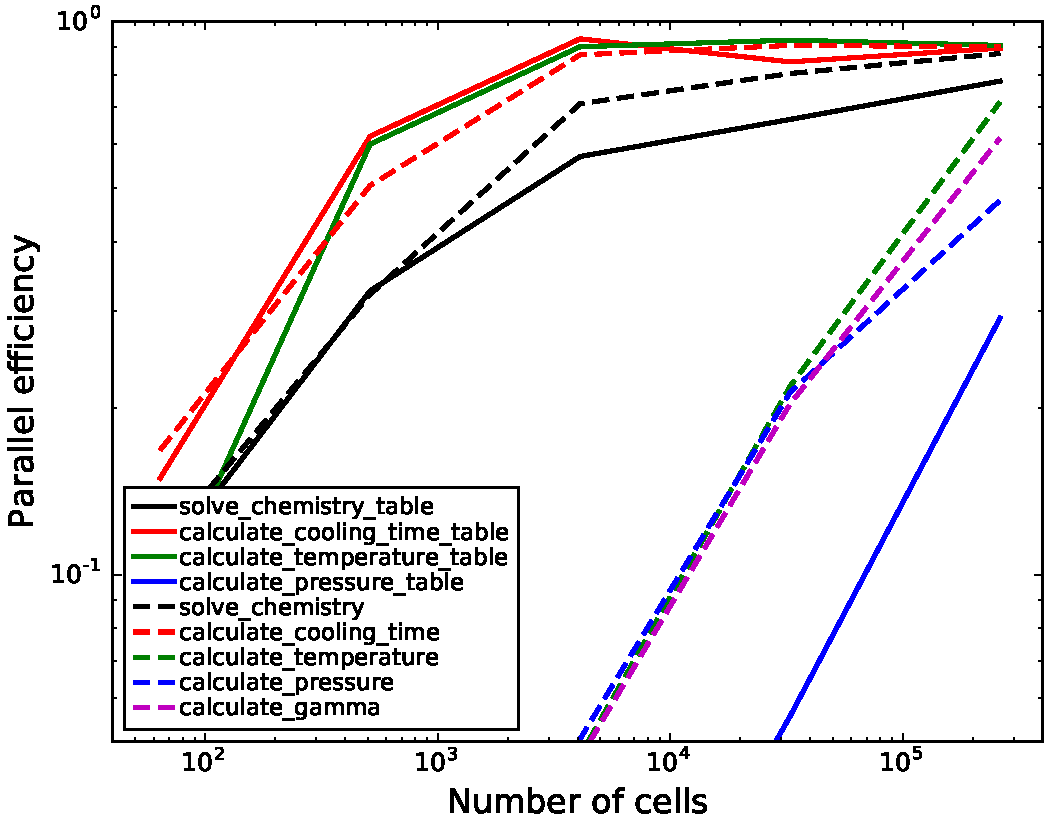
\includegraphics[width=0.84\textwidth]{fig__openmp_performance.pdf}
  \caption{
    OpenMP parallel efficiency using 20 threads as a function of the size of
    the input array. The solid and dashed lines are for the tabulated and
    non-equilibrium functionality, respectively. For all time-consuming
    routines, the parallel efficiency reaches $\sim 60\%\,\text{--}\,90\%$
    for $16^3$ cells and $\sim 80\%\,\text{--}\,90\%$ for $64^3$ cells.
  } \label{fig:omp-perf}
\end{figure*}
